\documentclass[10pt,letterpaper,notitlepage]{article}
\usepackage[utf8]{inputenc}
\usepackage{amsmath}
\usepackage{amsfonts}
\usepackage{amssymb}
\usepackage{graphicx}
\usepackage{cancel}
\usepackage{float}
\usepackage{cite}

\usepackage[ruled,vlined]{algorithm2e}


\usepackage[left=0.75in, right=0.75in, bottom=1.0in,top=0.75in]{geometry}

%\usepackage{caption} 
%\captionsetup[table]{skip=10pt}
%\usepackage[font=small,labelfont=bf]{caption}

\usepackage{comment}
\usepackage{listings}

\usepackage{color}
\definecolor{Brown}{cmyk}{0,0.81,1,0.60}
\definecolor{OliveGreen}{cmyk}{0.64,0,0.95,0.40}
\definecolor{CadetBlue}{cmyk}{0.62,0.57,0.23,0}

\usepackage{multicol}

\usepackage{appendix}

\usepackage{fancyhdr}
%\usepackage[colorlinks=true,linkcolor=blue,urlcolor=black,bookmarksopen=true,bookmarks]{hyperref}
\usepackage{bookmark}


%============================= Put document title here
\newcommand{\DOCTITLE}{Xenon-Iodine interaction programming assignment}  

%=============================  Load list of user-defined commands
% Mark URL's
\newcommand{\URL}[1]{{\textcolor{blue}{#1}}}
%
% Ways of grouping things
%
\newcommand{\bracket}[1]{\left[ #1 \right]}
\newcommand{\bracet}[1]{\left\{ #1 \right\}}
\newcommand{\fn}[1]{\left( #1 \right)}
\newcommand{\ave}[1]{\left\langle #1 \right\rangle}
\newcommand{\norm}[1]{\Arrowvert #1 \Arrowvert}
\newcommand{\abs}[1]{\arrowvert #1 \arrowvert}
%
% Derivative forms
%
\newcommand{\dxdy}[2]{\frac{\partial #1}{\partial #2}}
\newcommand{\dxy}[2]{\frac{d #1}{d #2}}
\newcommand{\dydx}[1]{\frac{\partial #1}{\partial x}}
\newcommand{\dydt}[1]{\frac{\partial #1}{\partial t}}
\newcommand{\dxdz}[1]{\frac{\partial #1}{\partial z}}
\newcommand{\dfdt}[1]{\frac{\partial}{\partial t} \fn{#1}}
\newcommand{\dfdz}[1]{\frac{\partial}{\partial z} \fn{#1}}
\newcommand{\ddt}[1]{\frac{\partial}{\partial t} #1}
\newcommand{\ddz}[1]{\frac{\partial}{\partial z} #1}
\newcommand{\dd}[2]{\frac{\partial}{\partial #1} #2}
\newcommand{\ddx}[1]{\frac{\partial}{\partial x} #1}
\newcommand{\ddy}[1]{\frac{\partial}{\partial y} #1}
\newcommand{\dxdyn}[3]{\frac{\partial ^{#3} #1 }{\partial #2 ^{#3}}}
\newcommand{\Dxdy}[2]{\frac{D #1}{D #2}}
\newcommand{\Dxy}[2]{\frac{D #1}{D #2}}
%
% Bold quantities
% 
\newcommand{\Omegabf}{\mathbf{\Omega}}
\newcommand{\bnabla}{\boldsymbol{\nabla}}
\newcommand{\position}{\mathbf{x}}
\newcommand{\dotp}{\boldsymbol{\cdot}}
%
% Vector forms
%
\renewcommand{\vec}[1]{\mbox{$\stackrel{\longrightarrow}{#1}$}}
\renewcommand{\div}{\mbox{$\vec{\mathbf{\nabla}} \cdot$}}
\newcommand{\grad}{\mbox{$\vec{\mathbf{\nabla}}$}}
\newcommand{\bb}[1]{\bar{\bar{#1}}}
%
% Vector forms boldfaced
\newcommand{\bvec}[1]{\mathbf{#1}}
\newcommand{\bdiv}{\boldsymbol{\nabla} \boldsymbol{\cdot}}
\newcommand{\bgrad}{\bnabla}
\newcommand{\mat}[1]{\bar{\bar{#1}}}
%
%
% Equation beginnings and endings
%
% Un-numbered equation with alignment
\newcommand{\beq}{\begin{equation*} \begin{aligned}}
\newcommand{\eeq}{\end{aligned}\end{equation*}}
% Numbered equation with alignment
\newcommand{\beqn}{\begin{equation}\begin{aligned}}
\newcommand{\eeqn}{\end{aligned}\end{equation}}  

% Numbered equation array, aligned	
\def\bea#1\eea{\begin{align}#1\end{align}}

\newcommand{\beas}{\begin{eqnarray*}}
\newcommand{\eeas}{\end{eqnarray*}}
\newcommand{\bdm}{\begin{displaymath}}
\newcommand{\edm}{\end{displaymath}}
%
% Equation punctuation
%
\newcommand{\pec}{\, ,}
\newcommand{\pep}{\, .} 
\newcommand{\pev}{\hspace{0.25in}}
%
% Equation labels and references, figure references, table references
%
\newcommand{\lequ}[1]{\label{eq:#1}}
\newcommand{\equ}[1]{Eq.~(\ref{eq:#1})}
\newcommand{\equs}[1]{Eqs.~(\ref{eq:#1})}
\newcommand{\requ}[1]{(\ref{eq:#1})}
\newcommand{\lfig}[1]{\label{fi:#1}}
\newcommand{\fig}[1]{Fig.~\ref{fi:#1}}
\newcommand{\figs}[1]{Figs.~\ref{fi:#1}}
\newcommand{\rfig}[1]{\ref{fi:#1}}
\newcommand{\lta}[1]{\label{ta:#1}}
\newcommand{\ta}[1]{Table~\ref{ta:#1}}
\newcommand{\rta}[1]{\ref{ta:#1}}
\newcommand{\lsec}[1]{\label{sec:#1}}
\newcommand{\rsec}[1]{\ref{sec:#1}}
%
% Superscript and subscript in text
%
\newcommand{\supertext}[1]{\ensuremath{^{\textrm{#1}}}}
\newcommand{\subtext}[1]{\ensuremath{_{\textrm{#1}}}}
%
% List beginnings and endings
%
\newcommand{\bl}{\bss\begin{itemize}}
\newcommand{\el}{\vspace{-.5\baselineskip}\end{itemize}\ess}
\newcommand{\ben}{\bss\begin{enumerate}}
\newcommand{\een}{\vspace{-.5\baselineskip}\end{enumerate}\ess}
%
% Figure and table beginnings and endings
%
\newcommand{\bfg}{\begin{figure}}
\newcommand{\efg}{\end{figure}}
\newcommand{\bt}{\begin{table}}
\newcommand{\et}{\end{table}}
%
% Tabular and center beginnings and endings
%
\newcommand{\bc}{\begin{center}}
\newcommand{\ec}{\end{center}}
\newcommand{\btb}{\begin{center}\begin{tabular}}
\newcommand{\etb}{\end{tabular}\end{center}}
%
% Single space command
%
\newcommand{\bss}{\begin{singlespace}}
\newcommand{\ess}{\end{singlespace}}
%
% Quick commands for symbols
%
\newcommand{\half}{\frac{1}{2}}
\newcommand{\third}{\frac{1}{3}}
\newcommand{\twothird}{\frac{2}{3}}
\newcommand{\fourth}{\frac{1}{4}}
\newcommand{\sixth}{\frac{1}{6}}
\newcommand{\mdot}{\dot{m}}
%\newcommand{\ten}[1]{\times 10^{#1}\,}
\newcommand{\cL}{{\cal L}}
\newcommand{\cD}{{\cal D}}
\newcommand{\cF}{{\cal F}}
\newcommand{\cE}{{\cal E}}
\renewcommand{\Re}{\mbox{Re}}
\newcommand{\Ma}{\mbox{Ma}}
\newcommand{\mA}{\mathbf{A}}
\newcommand{\mB}{\mathbf{B}}
\newcommand{\mC}{\mathbf{C}}
\newcommand{\E}{\mathcal{E}}
\newcommand{\F}{\mathcal{F}}
\newcommand{\Q}{\mathcal{Q}}
\newcommand{\U}{\mathbf{U}}
\renewcommand{\H}{\mathbf{H}}
\newcommand{\R}{\mathbf{R}}
\newcommand{\SN}{S$_{n}\,$}
\newcommand{\Flux}{\mathbf{F}}
\newcommand{\dt}{\Delta t}
\newcommand{\dx}{\Delta x}
\newcommand{\iL}{_{i,L}}
\newcommand{\iR}{_{i,R}}
\newcommand{\sa}{\sigma_a}
\newcommand{\sigsL}{\frac{\sigma_{s,i,L}^k}{2}}
\newcommand{\sigsR}{\frac{\sigma_{s,i,R}^k}{2}}
\newcommand{\sigtL}{\sigma_{t,i,L}^k}
\newcommand{\sigtR}{\sigma_{t,i,R}^k}
\newcommand{\halfh}{\frac{h_i}{2}}
\newcommand{\CN}[3]{\half\left[#1\right]^#2 + \half\left[#1\right]^#3}
\newcommand{\CNN}[3]{\half\left[#1\right]^#2 - \half\left[#1\right]^#3}
\newcommand{\BDF}[4]{\sixth\left[#1\right]^{#2} + \sixth\left[#1\right]^{#3} + \twothird\left[#1\right]^{#4}}
%
% More Quick Commands
%
\newcommand{\bi}{\begin{itemize}}
\newcommand{\ei}{\end{itemize}}
\newcommand{\dxi}{\Delta x_i}
\newcommand{\dyj}{\Delta y_j}
\newcommand{\ts}[1]{\textstyle #1}

\newcommand{\jcr}[1]{\textcolor{magenta}{#1}}
\usepackage[normalem]{ulem}
\newcommand{\ssout}[1]{\sout{\textcolor{magenta}{#1}}}

%
% Code syntax highlighting
%
%\lstset{language=C++,frame=ltrb,framesep=2pt,basicstyle=\linespread{0.8} \small,
%	keywordstyle=\ttfamily\color{OliveGreen},
%	identifierstyle=\ttfamily\color{CadetBlue}\bfseries,
%	commentstyle=\color{Brown},
%	stringstyle=\ttfamily,
%	showstringspaces=true,
%	tabsize=2,}

\lstset{language=C++,frame=ltrb,framesep=8pt,basicstyle=\linespread{0.8} \Large,
commentstyle=\ttfamily\color{OliveGreen},
keywordstyle=\ttfamily\color{blue},
identifierstyle=\ttfamily\color{CadetBlue}\bfseries,
stringstyle=\ttfamily,
tabsize=2,
showstringspaces=false,
numbers=left,
captionpos=t}

\renewcommand{\lstlistingname}{\textbf{Code Snippet}}% Listing -> Code Snippet


\begin{document}
\noindent
{\LARGE\textbf{\DOCTITLE}}
\newline
\newline
\newline
\noindent
{\Large Jan I.C. Vermaak$^{1,2}$}
\newline
\noindent\rule{\textwidth}{1pt}
{\small $^1$Center for Large Scale Scientific Simulations, Texas A\&M Engineering Experiment Station, College Station, Texas, USA.}
\newline\noindent
{\small $^2$Nuclear Engineering Department, Texas A\&M University, College Station, Texas, USA.}
\newline
\newline
\textbf{Abstract:}\newline\noindent
A simple ODE is used to describe the ${^{135}}$Xe and ${^{135}}$I transient behavior during steady operation of a reactor and directly after shutdown. We present the simplified equations and apply an appropriate temporal discretization that can be programmed.
\newline
\newline\noindent
{\small
\textbf{Keywords:} coupled ODE, explicit Euler}

\section{Introduction}
The localized behavior of ${^{135}}$Xe and ${^{135}}$I can generally be described by the following:
\begin{subequations}
\beqn 
\dxdy{N_X}{t} = \gamma_X N_{35} \sigma_f \phi  - \lambda_X N_X - N_X \sigma_{a,X} \phi + \lambda_I N_I
\eeqn 
\beqn 
\dxdy{N_I}{t} = \gamma_I N_{35} \sigma_f \phi - \lambda_I N_I,
\eeqn 
\beqn 
N_X(t=0) = N_I(t=0) = 0.0
\eeqn 
\end{subequations}
\newline 
\newline
where the subscripts $_X$ and $_I$ denote quantities for ${^{135}}$Xe and ${^{135}}$I respectively, $\gamma$ is the fission yield, $\lambda$ is the decay constant, $N$ is the atom density. $N_{35}$ is the fuel atomic density, $\sigma_f$ is the fuel's microscopic cross section for fission, $\sigma_{a,X}$ is $^{135}$Xe's absorption microscopic cross section, finally $\phi$ is the thermal neutron flux.

\section{Explicit Euler temporal discretization}
The explicit Euler temporal discretization can be described in simple terms by regarding the above set of coupled ODEs as a simplified set described by:
\beqn 
\dxdy{\mathbf{N}}{t} = \mathbf{F}(\mathbf{N},t)
\eeqn 
where $\mathbf{N}$ is a list/vector of time-dependent unknowns and $\mathbf{F}$ is function dependent both on the unknowns and time, $t$. The \textbf{explicit Euler} method then becomes
\beqn 
\frac{\mathbf{N}^{n+1} - \mathbf{N}^n}{\Delta t} &= \mathbf{F}(\mathbf{N}^n,t^n) \\
\mathbf{N}^0 &= \mathbf{N}(t=0)
\eeqn 
where the indices $n$ now denote the discrete time values of both time and all the unknowns.
\newline
\newline
Applying this scheme to our equations gives
\beqn \label{eq:discretized_eqs}
N_X^{n+1} &= N_X^n + \Delta t \biggr(
\gamma_X N_{35} \sigma_f \phi  - \lambda_X N_X^n - N_X^n \sigma_{a,X} \phi + \lambda_I N_I^n
\biggr) \\
N_I^{n+1} &= N_I^n + \Delta t \biggr(
\gamma_I N_{35} \sigma_f \phi - \lambda_I N_I^n
\biggr),
\eeqn 

\section{Assigment}
\textbf{Part 1}. Write a program that solves these equations for the following conditions:
\beq
\gamma_X  &= 0.00237 \\
\gamma_I  &= 0.0475 \\
\lambda_X &= 2.09e{-}5 \\
\lambda_I &= 2.87e{-}5 \\
\sigma_f  &= 500e{-}24 \\
\sigma_a  &= 1.0e6*1.0e{-}24  \\
N_{35}     &= 0.0077e24  \\
\phi      &= 1.0e14 \\
\Delta t  &= 2000.0 \\
\text{Total time} &= 300 \Delta t
\eeq 
\newline
\newline
Additionally, $N_X(t{=}0)=N_I(t{=}0)=0.0$, and at time $t>150\Delta t$, $\phi=0$.
\newline
\newline
\textbf{Part 2}. At each time step, including $n{=}0$, write the time $t$, the atomic densities $N_X$ and $N_I$ to a line in a text file. Each line of the file must contain 3 values separated by one or more spaces. For example:
\begin{verbatim}
0 0 0
2000 1.8249e+15 3.6575e+16
4000 5.30794e+15 7.10506e+16
6000 9.92769e+15 1.03547e+17
8000 1.52957e+16 1.34179e+17
10000 2.11239e+16 1.63052e+17
12000 2.72003e+16 1.90268e+17
14000 3.33695e+16 2.15921e+17
16000 3.95195e+16 2.40102e+17
18000 4.55705e+16 2.62896e+17
20000 5.14666e+16 2.8438e+17
etc.
\end{verbatim}

\textbf{Part 3}. Write a python script that can read the output file and automatically create a plot of the following nature:
\begin{center}
	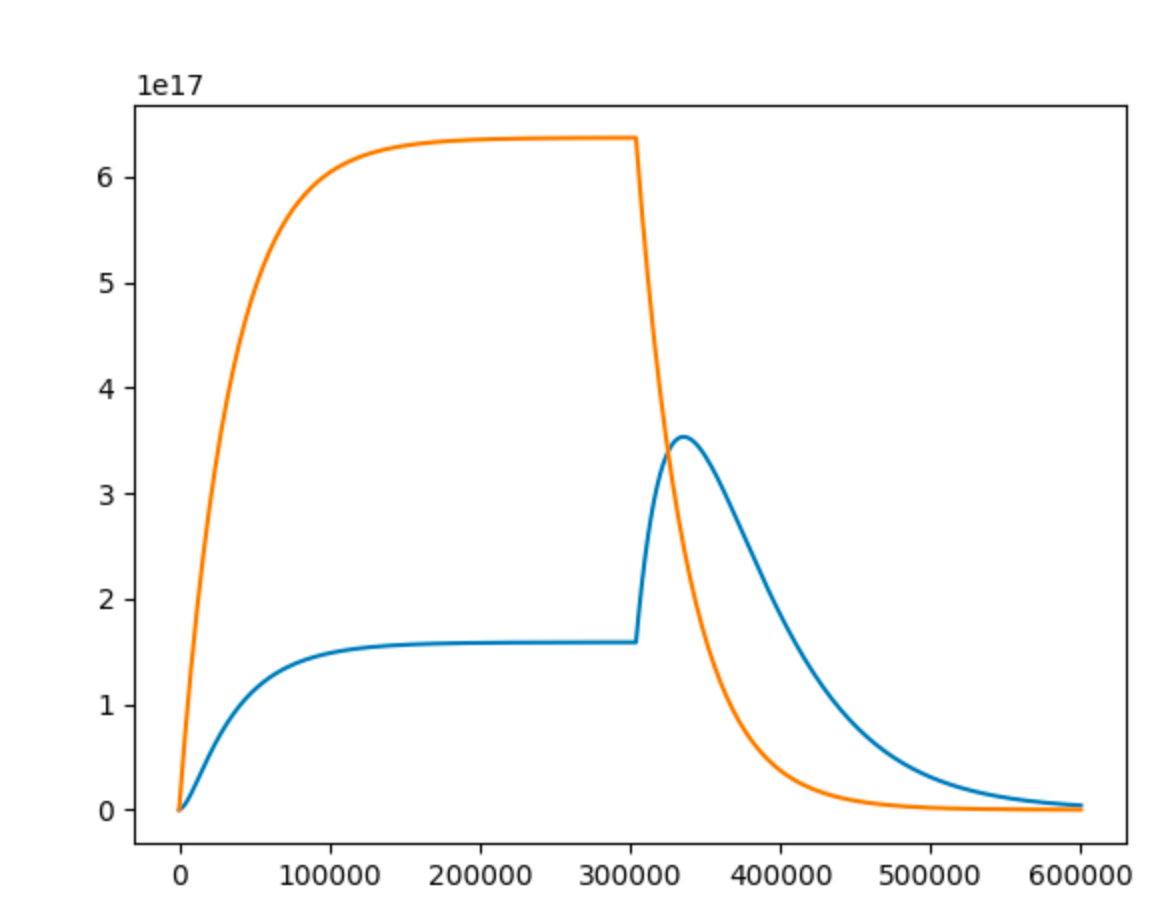
\includegraphics[width=0.4\linewidth]{screenshot001.png}
\end{center}


 
%\begin{thebibliography}{1}
%	
%	\bibitem{LewisMiller} Lewis E.E., Miller W.F., {\em Computational Methods of Neutron Transport}, JohnWiley \& Sons, 1984
%	   
%\end{thebibliography}

%\newpage
%\begin{appendices}
%\section{First appendix}
%Put ``Lazy reader stuff here".
%\end{appendices}

\end{document}